\section{Characteristics for Comparators}

\subsection{Input referred noise}
The goal is to find the sigma of a supposed normal distribution (Transient Noise simulations). If inputs are at the same potential there is equal probability of having "0s" (n0) and "1s" (n1). Differential input slightly skewed to have different n0 and n1. In this example: n1>n0

\begin{equation}
    \frac{n_0}{n_1} = \frac{\int_{-\infty}^{-Vs} f_x(x)dx}{1 - \int_{-\infty}^{-Vs} f_x(x)dx} \tag{5.10}
\end{equation}

When $Vs = \sigma$, then $n_0 = \frac{1 - 0.683}{2} = 0.1585$, $n_1 = 0.8415$. Measure Cumulative noise distribution then fit to gaussian distribution. After that, you can get sigma directly using MATLAB.

\begin{figure}[h]
    \centering
    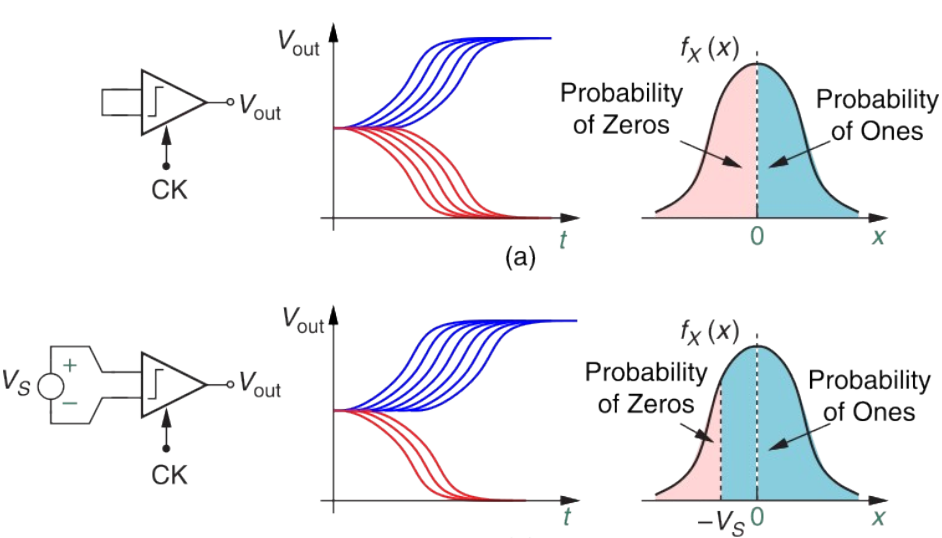
\includegraphics[width=0.6\textwidth]{img/DFE_img/DFE_img_37.png}
    \caption{The behavior of noisy comparator with a (a) zero and (b) finite input differences}
\end{figure}

\subsection{ISF (Impulse Sensitivity Function)}

Ideally, sampling is represented by a delta function $\delta$(t), where the value depends solely on the exact sampling time. In reality, however, a switch is modeled as a device that calculates a weighted average of the input signal over a finite duration, effectively treating the sampling function as a weighting function.

\textbf{Aperture delay:} the time elapsed from the sampling edge of the clock to the actual moment when the sample is taken, i.e., the middle of the aperture window.

\textbf{Aperture time (aka, time resolution):} the width of the peak of the SF where 80\% of the sensitivity is confined.

One of the speed limiting factors of the sampling element is the time resolution of the sampling switch.

\begin{equation}
    w_{80} = t_{90} - t_{10} \tag{5.11}
\end{equation}

\begin{equation}
    0.1 = \int_{-\infty}^{t_{10}} h(\tau) d\tau \tag{5.12}
\end{equation}

\begin{equation}
    0.9 = \int_{-\infty}^{t_{90}} h(\tau) d\tau \tag{5.13}
\end{equation}

\begin{figure}[h]
    \centering
    \begin{minipage}{0.48\textwidth}
        \centering
        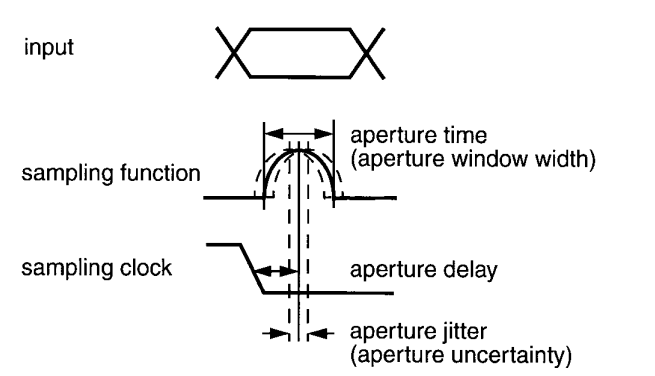
\includegraphics[width=.7\textwidth]{img/DFE_img/DFE_img_38.png}
        \caption{Some definitions of Sampling function \cite{johansson1998}}
    \end{minipage}
    \hfill
    \begin{minipage}{0.48\textwidth}
        \centering
        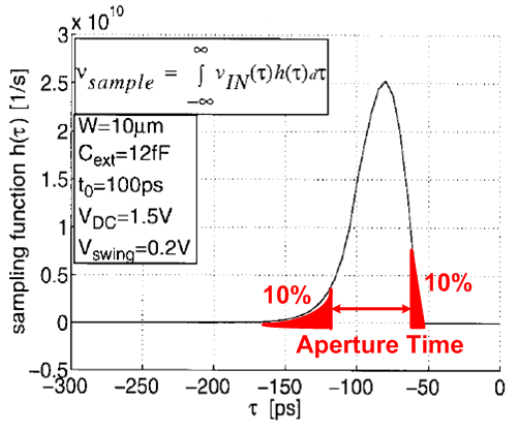
\includegraphics[width=.7\textwidth]{img/DFE_img/DFE_img_39.png}
        \caption{Plot of a sampling function h($\tau$) \cite{johansson1998}}
    \end{minipage}
\end{figure}


Comparator \textbf{ISF} is a subset of a time-varying impulse response h(t, $\tau$) for LTV systems:

\begin{equation}
    y(t) = \int_{-\infty}^{\infty} h(t, \tau) \cdot x(\tau) d\tau \tag{5.14}
\end{equation}

\textbf{h(t,$\tau$):} system response at t to a unit impulse arriving at $\tau$ where $\tau$ is the time shift between input and clock.

\begin{equation}
    ISF\ \Gamma(\tau) = h(t_{obs},\tau) \tag{5.15}
\end{equation}

For comparators, $t_{obs}$ is before decision is made output voltage of comparator.

ISF shows sampling aperture or timing resolution and also defines the setup time ($T_{setup}$) for DFE.

In frequency domain, it shows sampling gain and bandwidth.

\textbf{Sampling gain}: shows how strongly the input signal contributes to the output at the sampling instant.

\textbf{Sampling Bandwidth}: how fast the input sample can be distinguished.

\begin{figure}[h]
    \centering
    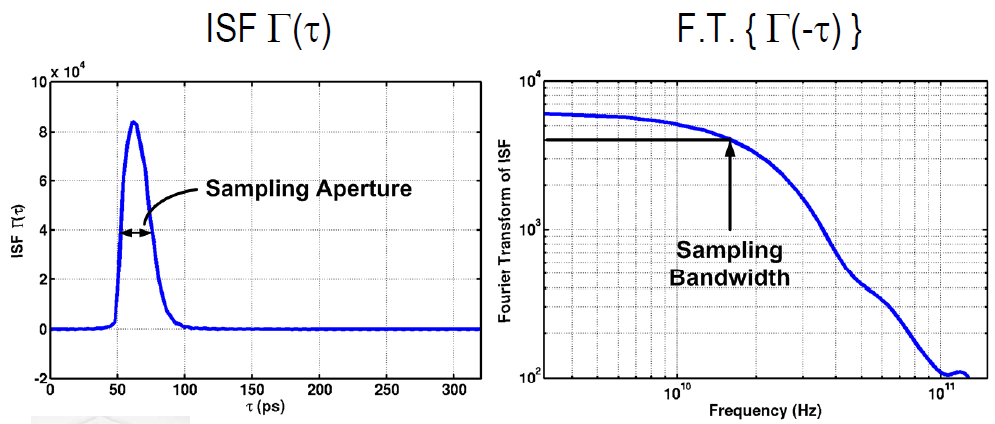
\includegraphics[width=0.7\textwidth]{img/DFE_img/DFE_img_40.png}
    \caption{(a) Impulse sensitivity function (ISF) of a clocked comparator indicating its sampling aperture. (b) The Fourier transform of the ISF indicating the sampling bandwidth. \cite{kim2009}}
\end{figure}

To characterize the ISF for a clocked comparator in simulation, one of the most famous ways in [ ].

- Characterizing Sampling Aperture of clocked Comparator
- Don't rely on accurate measurements of output voltage or using impulses
- Depends on metastability to get step sensitivity function then make derivative to ISF

\begin{figure}[h]
    \centering
    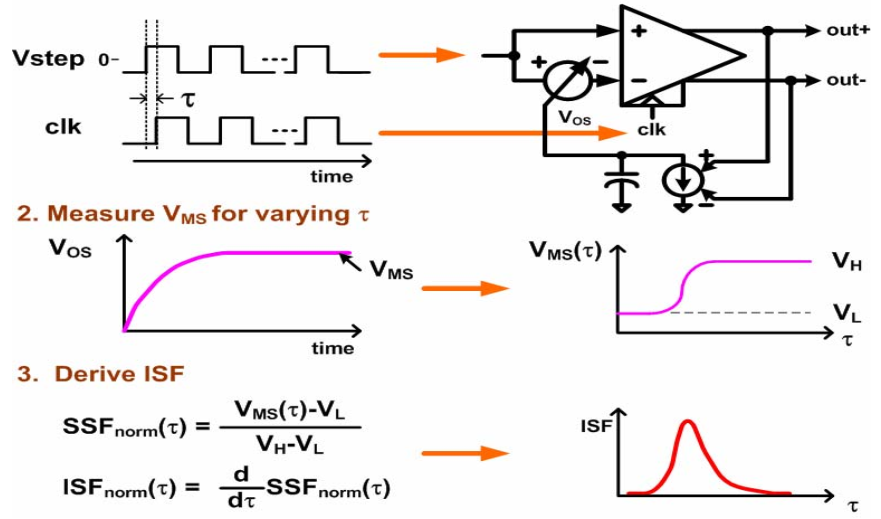
\includegraphics[width=0.6\textwidth]{img/DFE_img/DFE_img_41.png}
    \caption{Characterizing the comparator ISF in simulation \cite{johansson1998}}
\end{figure}

\section{Metastability}
For very small input voltages, the comparator cannot reach a decision in the limited time of a half clock period (Ts). The comparator will not generate a clear "zero" or "one" output level after time Ts (Metastability). The succeeding logical circuitry will behave ambiguously

Therefore, there is a spec on minimum input voltage for certain delay.

\begin{equation}
    V(t) = \Delta V_{in} e^{\frac{t}{\tau}} \rightarrow t_d = \tau \ln\frac{V(t_d)}{\Delta V_{in}} \tag{5.16}
\end{equation}

\begin{figure}[h]
    \centering
    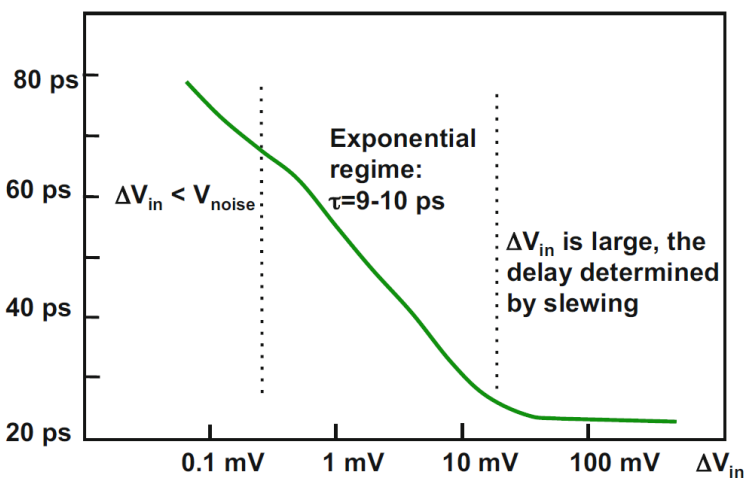
\includegraphics[width=0.5\textwidth]{img/DFE_img/DFE_img_42.png}
    \caption{Graph $T_{cq}$ vs $\Delta V_{in}$ \cite{pelgrom2017}}
\end{figure}